\subsection{Data-flow}
Il diagramma rappresenta il percorso dei dati all'interno del \textit{sistema}\textsubscript{\textit{G}} e le relative elaborazioni.

Vengono identificate le diverse entità coinvolte nel processo e le relazioni tra di esse, fornendo una panoramica dettagliata di come i dati vengono acquisiti, elaborati, archiviati e visualizzati.

\begin{figure}[H]
    \centering
    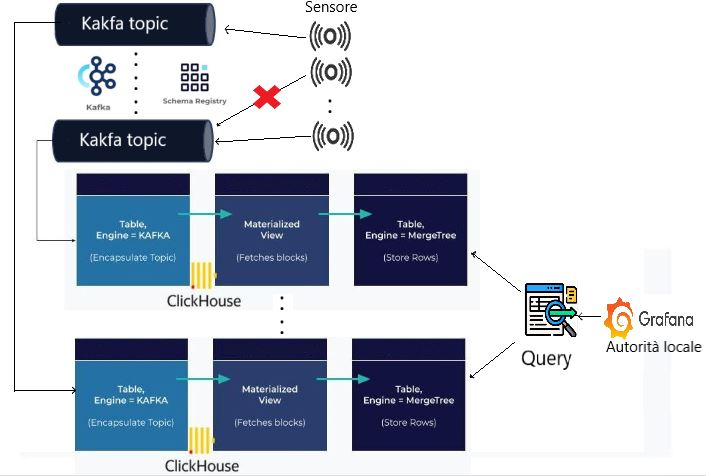
\includegraphics[width=1\textwidth]{../Images/SpecificaTecnica/data_flow.jpg}
    \caption{Data-flow - InnovaCity}
    \label{fig: dataflow}
\end{figure}

\begin{enumerate}
    \item \textbf{Generazione e invio dati:}
    \begin{itemize}
        \item I dati vengono generati dai simulatori dei sensori IoT e inviati al \textit{broker}\textsubscript{\textit{G}} \textit{Kafka}\textsubscript{\textit{G}}.
    \end{itemize}
    
    \item \textbf{Serializzazione e diramazione:}
    \begin{itemize}
        \item I dati vengono serializzati secondo lo schema definito nello schema registry per il relativo topic.
        Nel caso in cui il formato del messaggio non sia conforme a quanto definito nello schema registry questo viene scartato. A questo punto, il flusso si divide in due percorsi paralleli:
        \begin{enumerate}
            \item \textbf{Calcolo del punteggio di salute:}
            \begin{itemize}
                \item I dati di temperatura, umidità e polveri sottili vengono acquisiti dal processing layer per l'elaborazione;
                \item Il processing layer applica il modello di calcolo del punteggio di salute e reinvia i dati processati a un topic dedicato in \textit{Kafka}\textsubscript{\textit{G}};
                \item Lo schema registry verifica la validità del messaggio prima dell'invio.
            \end{itemize}
            
            \item \textbf{Archiviazione:}
            \begin{itemize}
                \item Le misurazioni (comprese sia quelle generate che quelle elaborate dallo \textit{stream processing}\textsubscript{\textit{G}}) fluiscono verso \textit{ClickHouse}\textsubscript{\textit{G}} tramite \textit{Kafka}\textsubscript{\textit{G}} engine e materialized view per l'archiviazione.
            \end{itemize}
        \end{enumerate}
    \end{itemize}
    
    \item \textbf{Visualizzazione:}
    \begin{itemize}
        \item I dati archiviati in \textit{ClickHouse}\textsubscript{\textit{G}} vengono interrogati da \textit{Grafana}\textsubscript{\textit{G}}, che genera visualizzazioni per la loro presentazione.
    \end{itemize}
\end{enumerate}
